\chapter{Solid-solid and Solid-fluid Heat Transfer in Solid Breeder Pebble Beds with Volume-Average Theory Modeling}\label{ch:cfd-dem-modeling-development}
Our DEM model, introduced in \Cref{ch:modeling-development}, was shown to be useful for modeling thermal transport between contacts in pebble beds in vacuum. The discrete element method's strength lies in its ability to resolve granular interactions at the pebble scale, allowing realistic modeling of contact forces and packing structure evolutions from crushed pebbles in fusion solid breeders. This is, however, insufficient on its own to model a solid breeder unit in a fusion reactor as the DEM equations neglect slow-moving helium purge gases permeating solid breeder pebble beds. Therefore, to develop a more complete model of temperature distributions in solid breeders, we will introduce the interstitial gas into our model.

Coupled granular-fluid flow is an important process used in a variety of industries.\cite{Zhou2010,Kloss2012} Early work on gas-particle flow models treated the solid and gas phases as two inter-penetrating continua. The solid and gas were treated with the so-called two fluid model (TFM) by Anderson \& Jackson as early as 1967.\cite{Anderson1967} Volume-averaging Theory (VAT) followed TFM. The VAT approach is similar to TFM in that the fluid computational cell is sufficiently large to include many individual particles but still smaller than the size of the system.\cite{Enwald1996} VAT allows treatment of complex porous flows with smooth continuous equations. In VAT, we average over a discrete space to replace complex geometry with a fictitious, smooth, continuous medium in which quantities of interest are defined independently of whether specific locations in that space are, for instance, solid or gas.\cite{Sbutega2013,whitaker1999method} The governing equations of VAT required constitutive equations for closure between the fluid and solid phases. To overcome the difficulties of closure in VAT, multi-scale strategies have been devised for formulation of governing equations and constitutive relationships between solid and fluid phase. 

At the microscopic level, the discrete element method describes the motion and energy transfer of particles interacting with a surrounding fluid. At the macroscopic level, fluid flow is handled in a continuum sense with volume-averaged governing equations that are closed with constitutive relationships with the particle phase.\cite{Tsuji1992,Xu1997} A numerical technique of coupling volume-averaged computational fluid dynamics (CFD) flow solvers to discrete element models was first proposed by Tsuji\etal. in 1992 and then Hoomans\etal~in 1996.\cite{Tsuji1992,Tsuji1993,Hoomans1996} Since then, CFD-DEM coupling approaches have grown as a tool for granular flow research and many CFD-DEM models have been experimentally validated for fluidized beds and preliminarily validated for heat transfer in packed beds.\cite{Kloss2012,Xu1997,Patankar2001,Swasdisevi2005,Deen2007,Zhang2008,Chu2008,VanBuijtenen2011,Gruber2012,Peng2014}


Noting the growth in application of coupled CFD-DEM, a systematic review of the theoretical developments behind different particular system models was given by Zhu\etal\cite{Zhu2007} They consider the two most common formulations, following the notation of Gidaspow, for the governing equations. The two formulations are commonly referred to simply as Model A and Model B.\cite{gidaspow1994multiphase} Both of these models have been implemented somewhat interchangeably in CFD-DEM simulations. As pointed out by Zhu\etal, the two models differ by their treatment of the pressure drop. In Model A, the pressure drop on the system is jointly shared by the gas and solid phases. In Model B, it is only the gas phase which directly experiences the effects of pressure drop. Therefore, the two models have different forms of coupling source term, $S_k$ (see \Cref{eq:cfd-mom-source}). The source of Model B is related to that of Model A as $S_k^B = S_k^A/\epsilon - \rho_f\phi g$.

However, as is shown by Zhou\etal, there is a built-in assumption to Model B which is typically overlooked in the implementation of CFD-DEM. For an accelerating fluid, there is an added-mass in the momentum equation. In the derivation of Model B, it is tacitly assumed that the fluid is steady which is not generally valid.\cite{Zhou2010} Nevertheless, the proliferation of Model B is due to the ease in numerical implementation and, except for some situations, Model B is numerically similar to Model A for most cases studied in CFD-DEM simulations.\cite{Zhou2010} In the simulations of packed beds for tritium breeding, we choose to implement Model B as it is valid for any of the flow scenarios ever experienced by the ceramic pebble bed.

 
 

%%%%%%%%%%%%%%%%%%%%%%%%%%%%%%%%%%%%%%%%%%%%%%%%%%%%%%%%%%%%%%%%%%%%%%%%%%%%%%%%%%%%%%%%%%%%%%%%%%%%%%%%%%%%
%%%%%%%%%%%%%%%%%%%%%%%%%%%%%%%%%%%%%%%%%%%%%%%%%%%%%%%%%%%%%%%%%%%%%%%%%%%%%%%%%%%%%%%%%%%%%%%%%%%%%%%%%%%%
%
% new section
%
%%%%%%%%%%%%%%%%%%%%%%%%%%%%%%%%%%%%%%%%%%%%%%%%%%%%%%%%%%%%%%%%%%%%%%%%%%%%%%%%%%%%%%%%%%%%%%%%%%%%%%%%%%%%
%%%%%%%%%%%%%%%%%%%%%%%%%%%%%%%%%%%%%%%%%%%%%%%%%%%%%%%%%%%%%%%%%%%%%%%%%%%%%%%%%%%%%%%%%%%%%%%%%%%%%%%%%%%%
\section{Modeling Particles in the Presence of Fluid Flow Fields} \label{sec:modeling-cfd-dem}
Governing equations of DEM systems were given in \cref{sec:particle-dynamics}. To review, each pebble obeys Newton's equations of motion in response to a net force acting upon it. To include the influence of helium in the DEM formulation, we simply add a drag force term to \Cref{eq:newton-translational}. The momentum balance of our Lagrangian-tracked pebble now reads,
\begin{equation}\label{eq:cfdem-dem-momentum}
	m_i  \ddt{\vec{r}_i} = m_i\vec{g} + \vec{f}_i + \beta_i V_i \Delta \vec{u}_{if}
\end{equation}
The components of the last term are $\Delta \vec{u}_{if} = \vec{u}_f - u_i$, which is the relative velocity between the fluid and pebble, $i$; $\beta_i$, a volumetric drag coefficient; and the drag acts upon the entire pebble volume, $V_i$. A discussion on the method of determination and form of the inter-phase drag coefficient will be discussed after introducing the DEM heat transfer equation.

To similarly include the influence of helium gas field surrounding pebble, $i$, on its temperature, we must simply add a source term to the original energy balance equation of the DEM pebble, as given in \Cref{eq:thermoFirstLaw}. In this case, the inter-phase exchange coefficient for energy is the heat transfer coefficient, $h$, for a fluid moving past a sphere in a packed bed. Heat transfer with passing fluids is added to the energy balance as
\begin{equation}\label{eq:cfdem-dem-energy}
	m_iC_i \ddt{T_i} = Q_{s,i} + \sum_{j=1}^Z Q_{ij} + h_i A_i \Delta T_{if}
\end{equation}
where again we have only needed to add the last term to account for the energy deposited/removed by the passing fluid. $\Delta T_{if}$ is the temperature difference, $T_f - T_i$, and the inter-phase energy exchange coefficient, $h_i$, acts upon the pebble surface area, $A_i$.

In the development of \Cref{eq:thermoFirstLaw}, it was assumed that a `conduction' Biot number was satisfied such that a lumped-capacitance method would be valid for the discrete pebbles in our ensemble. Likewise, for \Cref{eq:cfdem-dem-energy} to be valid, we must assume that the true Biot number is also $\Bi \ll 1$. However, the lumped capacitance method is generally developed in heat transfer systems without heat generation. Furthermore, considering the low conductivity of our pebble material, it is not apparent \textit{a priori} if the lumped capacitance assumption inherent in our DEM formulation is valid. The validity of the assumption is explored in \cref{sec:ht-jeffreson-correction}.

At present, assuming their validity, these simple additions to the governing equations of momentum and energy of each particle are all that are necessary to incorporate helium into the DEM computations of solid breeder pebbles. The computations of the inter-phase exchange coefficients, $\beta_i$ and $h_i$ are discussed next.

\subsection{Inter-phase Exchange Coefficients}

The purge gas in ceramic breeders is meant to travel at very low flow rates to maximize the absorption of tritium. The pebble beds will also always be near the close-packed limit. As such, the particle Reynolds number for these flows is often near unity and the Kozeny-Carman equation, as applicable for Stokes flow, is quite sufficient. However, we will employ the full Koch-Hill-Ladd (KHL) correlations which include terms for both the Stokes flow correlation (as a function of $\phi$) in the zero Reynolds number limit and the viscous effects with a Reynolds number-dependent term. The KHL correlation is of a general form, and reduces to the Kozeny-Carman correlation in the close-packed, zero Reynolds number limits.\cite{Koch2001} The KHL correlation allows for flexibility of discretized fluid cells to contain low volume-fraction regions of pebble beds, such as in the near-wall region. A short review of other correlations, their applicable ranges of fluid parameters, and other details is given in \cref{sec:modeling-pressure-drop}. The assumptions leading to the development of the KHL correlation provide justification for our implementation in packed beds of lithium ceramics.

The nondimensional force of the KHL correlation reads,
\begin{equation}\label{eq:khl-correlation}
	F = F_0(\phi) + F_3(\phi)\Re
\end{equation}
where the viscous term of the drag is
\begin{equation}
F_0 = \begin{cases}
	\frac{1+3(\phi/2)^{1/2} + (135/64)\phi\ln\phi + 16.14\phi}{1 + 0.681\phi - 8.48 \phi^2 + 8.16\phi^3} & \text{if $\phi < 0.4$}\\
	10.0\,\frac{\phi}{(1-\phi)^3} & \text{if $\phi > 0.4$} 
	\end{cases}
\end{equation}
and the inertial component of the drag is
\begin{equation}
	F_3 = 0.0673 + 0.212\phi + 0.0232 \frac{1}{(1-\phi)^5}
\end{equation}

The correlation from Koch-Hill-Ladd provide a nondimensional drag that must simply be re-written to fit into the pattern of our inter-phase momentum exchange coefficient. The momentum exchange coefficient follows the common form by Gidaspow.\cite{gidaspow1994multiphase} The form used here is actually that of Van der Hoef, which differs from the classic form of Gidaspow by a factor of $1-\phi$, because numerically it is more convenient to couple the pressure gradient force to the buoyancy force.\cite{Hoef2005,Benyahia2006} Thus,
\begin{equation}\label{eq:interphase-momentum}
	\beta_{i} = \frac{18\mu_f}{d_{p,i}^2}(1-\phi_k)\phi_k F
\end{equation}
where $\mu_f$ is the fluid viscosity and the diameter of pebble $i$ is $d_{p,i}$. The packing fraction, $\phi_k$, in this equation is the local packing fraction in the fluid cell $k$. Localized packing fraction in a ceramic breeder volume may change in time due to fragmentation of pebbles or other packing rearrangement. The packing fraction will also change due to ordered packing enforced by pebble bed mechanical boundaries.\cite{Hunt1990,Benenati1962,Baird1958} For example, the void fraction ($\epsilon = 1-\phi$) in narrow annular containers using the correlation from Mueller, as a function of wall-distance in a cylinder is,\cite{Mueller1999}
\[
\epsilon = \epsilon_0 + (1-\epsilon_0)J_0(ar^*)e^{-br^*}
\]
where $r^*$ is the nondimensional distance from the wall; here it is defined in terms of the pebble diameter, $r^* = r/d_p$. The constants, a and b, are defined in terms of the size parameter $\alpha = D/d_p$ where $D$ is the diameter of the annular tube. First, $a$ is
\[
    a= 
\begin{cases}
    7.383 - \cfrac{2.932}{\alpha - 9.864}, & \text{if }\  \alpha \geq 13\\
    8.243 - \cfrac{12.98}{\alpha + 3.156}, & \text{if} \ 13 \geq \alpha \geq 2.61
\end{cases}
\]
then
\[
b = 0.304 - \cfrac{0.724}{\alpha}
\]
The bulk void fraction is found from the correlation:
\[
\epsilon_0 = 0.379 + \cfrac{0.078}{\alpha - 1.8}
\]


\begin{figure}[htbp]
\centering
	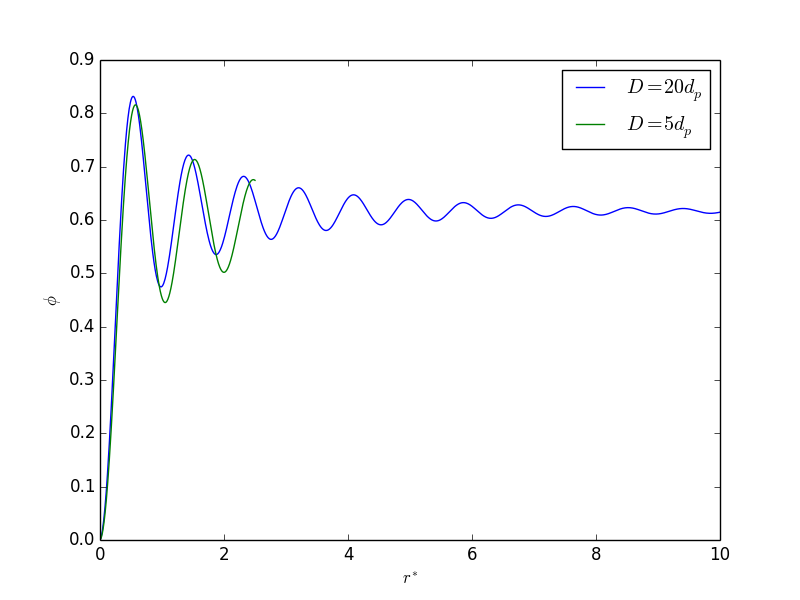
\includegraphics[width = \singleimagewidth]{figures/annular-packing-fraction.png}
	\caption{Showing the packing fraction approach the bulk value after a few pebble diameters when the pipe is 20$d_p$ and that when the pipe is only 5$d_p$, the packing fraction at any radius is not the same as the bed average.}
	\label{fig:packingDist}
\end{figure}

The packing fractions as a function of distance from the container wall for two example sizes, diameters of 20$d_p$ and 5$d_p$, are plotted in \Cref{fig:packingDist}. This example is meant to demonstrate the varying packing fraction in a packed bed that is described with a single `bulk' or `global' packing fraction. It is important that the computational cell used in the CFD domain be sufficiently small to capture the variation of void fraction in near-wall regions. The size of the discretized cell relative to the pebble will dictate how much of the void fraction variation is captured in the volume-averaged equations.




\FloatBarrier



The inter-phase energy transfer coefficient is calculated from the Nusselt number for the helium flow in the ensemble,
\begin{equation}\label{eq:interphase-energy}
	h_i = \frac{\Nu k_f}{d_{p,i}}
\end{equation}
where $k_f$ is the thermal conductivity of the fluid. Several correlations for determining the Nusselt number are given for reference in \cref{sec:particle-convection}. For the low-Reynolds number flows of the helium purge gas, the most appropriate correlation is from Wakao\etal, given in \Cref{eq:wakao}.
% We opt for the correlation provided by Li \& Mason which is applicable to a wide range of Reynolds number flows.\cite{Li2000} Their correlation reads,
% \begin{equation}\label{eq:li-mason-correlation}
% 	\Nu = \begin{cases}
% 	2+ 0.6\epsilon^n\Re_p^{1/2}\Pr^{1/3} 										& \Re_p < 200\\
% 	2+ 0.5\epsilon^n\Re_p^{1/2}\Pr^{1/3} + 0.02 \epsilon^n \Re_p^{0.8}\Pr^{1/3} & 200 < \Re_p < 1500\\
% 	2+ 0.000045\epsilon^n\Re_p^{1/2}			 								& \Re_p > 1500
% 	\end{cases}
% \end{equation}

% The correlation was developed for small spheres of polymer pellets in relatively dilute flow for which they found the exponent of the void fraction to be fit well to experiments when $n=3$. It might be argued that a different exponent might be necessary to apply this correlation to our packed beds. In practice, however, we observe that the majority of the Nusselt numbers calculated in each cell of the helium mesh are approximately $\Nu = 2$ which is the pure-conduction limit -- regardless of the exponent. For this reason, it is safe to assume $n=3$ is valid for our packed beds at this time.

From Eqs.~\ref{eq:interphase-momentum} and~\ref{eq:interphase-energy}, we have a formulation wherein knowledge of the flow field around our pebbles will allow calculation of dimensionless drag, $F$, and Nusselt number, $\Nu$,  and thereby the two inter-phase exchange coefficients. The flow is coupled to our DEM computations with simple algebraic additions to the equations of motion and energy of the pebble, \Cref{eq:cfdem-dem-momentum} and \Cref{eq:cfdem-dem-energy}, respectively.




\subsection{Volume-averaged Thermofluid Flow}

The gas phase flow field will be treated in a method analogous to the approach of volume-averaging theory (VAT); the criticl difference is that with formal VAT the solid field is not handled with the discrete element strategy employed in CFD-DEM models.\cite{Tsuji1992} 

In this formulation of gas flow, we discretize fluid space with cells that are slightly larger than the individual particles; in the application of our CFD-DEM coupling, this meant at most roughly 5 to 6 particles per cell. With VAT, the particles themselves are not resolved in the fluid space but are simply introduced \textit{via} closure terms.\cite{Sbutega2013,Horvat2006} A clear derivation of the governing equations of VAT can be found in Sbutega\etal.\cite{Sbutega2013} The momentum and energy of a fluid flow through a solid phase with volume-averaged Navier-Stokes and energy equations are applied to each cell, $k$, in the discretized fluid space,
\begin{subequations}\label{eq:cfd-equations}
\begin{align}
\pder[\epsilon_k \rho_f]{t} + \nabla\cdot(\epsilon_k \vec{u}_f \rho_f) &= 0\\
\pder[\epsilon_k \vec{u}_f]{t} + \nabla\cdot(\epsilon_k \vec{u}_f \vec{u}_f) &= -\frac{\epsilon_k}{\rho_f}\nabla P_f + \nabla\cdot\left(\nu_f\epsilon_k\nabla \vec{u}_f\right) - \frac{S_k}{\rho_f}\\
\pder[\epsilon_k T_f]{t} + \nabla\cdot(\epsilon_k \vec{u}_f T_f) &= \nabla\left(\epsilon_k\nabla T_f\right)-\frac{E_k}{\rho_fC_f}
\end{align}
\end{subequations}
where the packing fraction in any fluid cell is calculated as a function of the volumes of particles residing in cell $k$. The computation of the void fraction is critically important and is discussed in length in \cref{sec:lag-eul-mapping}.
% \begin{equation}
% 	\phi_k = \frac{1}{V_k}\sum_{\forall i \in k} V_{p,i}
% \end{equation}
% where the fluid void fraction is the complement of the solid packing fraction, $\epsilon = 1 - \phi$. 

Coupling the fluid phase to the particles happens with the closure terms in momentum and energy of $S_k$ and $E_k$, respectively. They are volume-weighted sums of the drag forces and energy exchanges for all particles in the discretized fluid cell,

\begin{subequations}\label{eq:cfd-sources}
\begin{align}
	S_k &= \frac{1}{V_k}\sum_{\forall i \in k} \beta_i V_i \Delta \vec{u}_{if} \label{eq:cfd-mom-source}\\
	E_k &= \frac{1}{V_k}\sum_{\forall i \in k} h_i A_i \Delta T_{if}
\end{align}
\end{subequations}

The inter-phase momentum and energy exchange coefficients act as the communicators between the particle information from the DEM solver and the fluid fields from CFD. Thus the motion and energy of the fluid field are intimately and dynamically coupled with the particle positions and energy. Computational time is preserved by only considering volume-averaged values in the fluid domain but important inter-particle forces are still calculated in the DEM space. The nature of the coupling, \textit{i.e.} how information is mapped between the two computational spaces, is discussed next.%The cross-communication between fluid and solid is accomplished with a coupling routine that is explained in detail in Refs. 11, 12.





\subsection{Lagrangian-Eulerian Mapping Calculations of Porosity}\label{sec:lag-eul-mapping}

The simplest method for calculating the porosity of a CFD computational cell is to map all the DEM particles into the Eulerian volume \textit{via} their centroid. We refer to this simple technique as the particle centroid method; in spite of its simplicity it is often used for large cell-to-particle volume ratios.\cite{Xu1997} A two-dimensional demonstration of the centroid technique is given in \Cref{fig:centroid-void-fraction}. In this figure, we see a computational cell (dashed line) in which many particles exist either partially or fully. The particles shaded in red have their centers located inside the cell and therefore in the simple technique have their entire volume contribute to the calculation of the porosity. The porosity for the centroid method is calculated as,
\begin{equation}
	\epsilon_\text{cell} = 1-\frac{1}{V_\text{cell}}\sum_{i = A}^{i=L}V_{p,i}
\end{equation}
where $V_{p,i}$ is the volume of particle $i$. As the cell size begins to approach the size of the particle, erroneous calculations of porosity arise. This is visible, for instance, when considering particle $A$ in \Cref{fig:centroid-void-fraction}. This particle has only a quarter of its volume inside the cell but the porosity of the cell is computed as if the entire particle existed inside. Hoomans\etal~recognized this limitation of the centroid method and introduced a fractional volume method.\cite{Hoomans1996} In the fractional volume method, the porosity is found as only partial volumes of the original sphere,
\begin{equation}
	\epsilon_\text{cell} = 1-\frac{1}{V_\text{cell}}\sum_{i = A}^{i=L}f_iV_{p,i}
\end{equation}
where $f_i$ is the fraction of the particle residing in the Eulerian cell. A similar approach taken by Kloss\etal~and Zhao \& Shan is the divided technique.\cite{Kloss2012,Zhao2013a} In this technique, the spherical particle is artificially divided into a number of regions with markers indicating their location. For example, see now how particles at the boundary, such as particle $A$, are treated in \Cref{fig:centroid-void-fraction-divided}. Instead of searching for centroids of particles, each particle has a search through the marker points (the black markers drawn in particle $A$) and the volume of that section of the sphere is assigned to whichever cell it falls inside. Note that in the sketch of \Cref{fig:centroid-void-fraction-divided}, every particle is divided with markers but particles not near the cell boundary have not had them drawn for clarity and convenience.

\begin{figure}[ht]
	\centering
	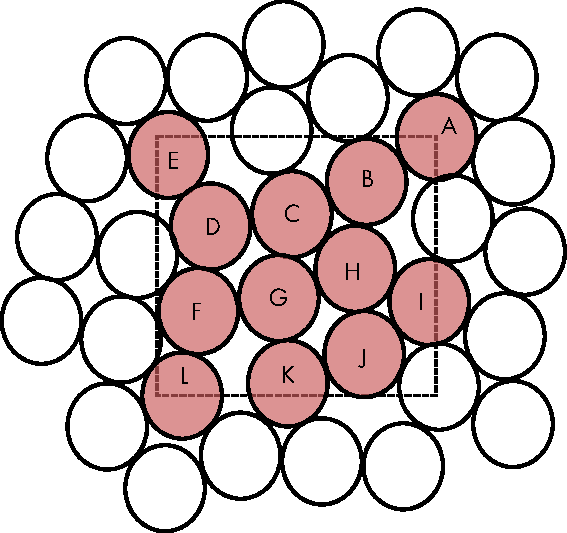
\includegraphics[width=\singleimagewidth]{figures/void-fraction-cell.pdf}
	\caption{The dashed line represents a computational cell in which exist many particles. The particles with centroids inside the cell are shaded red.}\label{fig:centroid-void-fraction}
\end{figure}

\begin{figure}[t]
	\centering
	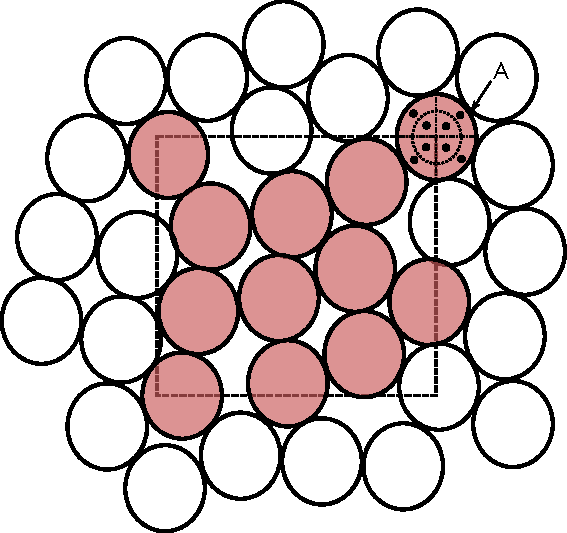
\includegraphics[width=\singleimagewidth]{figures/void-fraction-divided-cell.pdf}
	\caption{The dashed line represents a computational cell in which exist many particles. The divided portions of the particles with the sectional markers (dots) located in the cell are colored red.}\label{fig:centroid-void-fraction-divided}
\end{figure}

As the computational cell volume approaches the size of a single particle $V_\text{cell}\rightarrow V_p$, the centroid and divided techniques break down. A technique introduced by Link\etal~treats the particle as a porous cube and allows computations when a cell is completely occupied by only a single particle.\cite{Link2005} Peng\etal~offer an analytic technique as well as guidelines for validity of either analytic or centroid techniques.\cite{Peng2014} However, in this work, the divided technique of Kloss\etal~is implemented, based on the geometry of our packed bed flow and the guidelines established by Peng\etal\cite{Kloss2012,Peng2014}


\subsection{Eulerian-Lagrangian Mapping Calculations of Force and Energy}
Once the fluid momentum and energy fields are calculated in the Eulerian grid, the coupled inter-phase exchange coefficients must map the velocities and temperatures onto the particles in the Lagrangian DEM framework. A particle centroid method is always used in the exchange onto the particles. Referencing \Cref{fig:centroid-void-fraction}, the velocity and temperature of the dashed cell is mapped only onto the particles highlighted in red. The approach has been used successfully by others.\cite{Xu1997,Link2005,Kloss2012}



\subsection{Numerical Implementation of CFD-DEM}\label{sec:cfd-dem-solver}

The infrastructure for solving the DEM equations continues to be handled by LIGGGHTS. Details of the software are described in \cref{sec:dem-solver}. The DEM solver is a highly parallel C++ code based on the Molecular Dynamics (MD) code LAMMPS.\cite{Plimpton1995}

Taking advantage of a separate, stand-alone CFD solver that is maintained by a large community, the CFD simulations are conducted by the pressure-based solver using the PISO algorithm realized within the open-source framework of OpenFOAM\textsuperscript{\textregistered}.\cite{Issa1986,OpenCFDLtd2014} The coupling routines, maintained by DCS Computing GmbH, are collected in a library providing a modular framework for CFD-DEM coupling with the C++ codes LIGGGHTS and OpenFOAM\textsuperscript{\textregistered}.\cite{Kloss2012,Goniva2012}

% The helium purge gas generally flows at very small Reynolds numbers. Particle Reynolds numbers on the order of unity, $\Re\sim1$, are expected for many tritium breeding volumes. 

The routine of coupling CFD-DEM consists of several steps:
\begin{enumerate}
\item the DEM solver calculates the particles positions, velocities, and temperatures with time step dictated by stability of DEM
\item the particles positions and velocities are passed to the CFD solver using the Message Passing Interface (MPI)
\item for each particle, the cell in the CFD mesh that contains the particle is located
\item for each cell, the particle volume fraction is determined from the divided technique described in \cref{sec:lag-eul-mapping}. The ensemble-average velocity of the particles is determined
\item on the basis of $\epsilon$ and $\Re_p$, the fluid forces and heat transfer rate acting on each particle are calculated from the inter-phase exchange coefficients of Eqs.~\ref{eq:interphase-momentum} and~\ref{eq:interphase-energy}
\item the momentum and energy source/sink terms are assembled from particle-based forces by ensemble averaging over all particles in a CFD cell \textit{via} Eqs.~\ref{eq:cfd-sources}
\item the inter-phase exchange coefficients of Eqs.~\ref{eq:interphase-momentum} and~\ref{eq:interphase-energy} are sent to the DEM solver
\item the CFD solver calculates the fluid velocity and temperature from the source/sink terms determined in step 6.
\end{enumerate}

%%%%%%%%%%%%%%%%%%%%%%%%%%%%%%%%%%%%%%%%%%%%%%%%%%%%%%%%%%%%%%%%%%%%%%%%%%%%%%%%%%%%%%%%%%%%%%%%%%%%%%%%%%%%
%%%%%%%%%%%%%%%%%%%%%%%%%%%%%%%%%%%%%%%%%%%%%%%%%%%%%%%%%%%%%%%%%%%%%%%%%%%%%%%%%%%%%%%%%%%%%%%%%%%%%%%%%%%%
%
% new section
%
%%%%%%%%%%%%%%%%%%%%%%%%%%%%%%%%%%%%%%%%%%%%%%%%%%%%%%%%%%%%%%%%%%%%%%%%%%%%%%%%%%%%%%%%%%%%%%%%%%%%%%%%%%%%
%%%%%%%%%%%%%%%%%%%%%%%%%%%%%%%%%%%%%%%%%%%%%%%%%%%%%%%%%%%%%%%%%%%%%%%%%%%%%%%%%%%%%%%%%%%%%%%%%%%%%%%%%%%%
\section{Jeffreson Correction to Lumped Capacitance Method}\label{sec:ht-jeffreson-correction}
When incorporating helium into the DEM-based modeling, the lumped capacitance assumption for each particle in the ensemble is assumed. The assumption eases the computational efforts of solving for the temperature distribution inside each particle; each particle is treated as being isothermal. The accuracy of the lumped capacitance method is described by the Biot number,
\begin{equation}
     \Bi = \frac{hd_p}{k_r}
\end{equation} 
and for $\Bi \ll 1$ the lumped capacitance method accurately models the behavior of a solid interacting with a fluid. For $\Bi \approx 0.1$ (in cases with no heat generation), the error from the lumped capacitance method is only about 5\%. In solid breeder volumes, the particles are generally small, the solid conductivity low, and heat transfer coefficient generally is also low. This leads to small-to-moderate Biot numbers expected in the packed bed. In this section we will analyze the accuracy of the lumped capacitance and introduce a correction method to account for inaccuracies of the method at moderate Biot numbers.

I simplify the case of a packed bed and only consider a single sphere with volumetric heat generation submerged in- and thermally interacting with a fluid. The sphere will be of radius $R=d_p/2$, as shown in \Cref{fig:ParticleControlVolume}. The sphere will initially be at a uniform temperature of $T_i$. The fluid temperature will remain constant at $T_f$

\begin{figure}[ht]
	\centering
		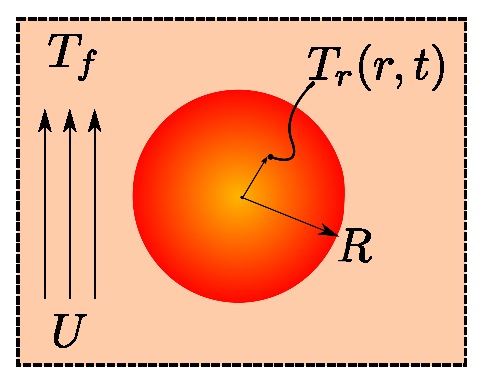
\includegraphics[width=2in]{figures/ParticleControlVolume}
	\caption[Control volume of single spherical particle in a packed bed]{Control volume of a single spherical particle in a packed bed}
	\label{fig:ParticleControlVolume}
\end{figure}


%~~~~~~~~~~~~~~~~~~~~~~~~~~~~~~~~~~~~~~~~~~~~~~~~~~~~~~~
\subsection{Lumped Capacitance Solution for Sphere}\label{sec:lumped-capacitance}
I solve for a single sphere interacting with a passing fluid, as shown in \Cref{fig:ParticleControlVolume}, while making the lumped capacitance assumption for this sphere. The solid is initially at temperature $T_0$, with constant volumetric heat generation, cooling in a fluid with constant heat transfer coefficient. The fluid will remain constant at $T_f$.

The time response of the sphere's temperature is dictated by the balance of energy to/away from the solid,  

\begin{equation}\label{eq:lc-energy-balance}
	\rho_rC_rV\frac{dT}{dt} = -hA(T-T_f) + \dot{g}V
\end{equation}

\Cref{eq:lc-energy-balance} is solved in dimensionless form with the following nondimensional parameters of temperature and time,
\begin{subequations}
\begin{align}
    \theta &= \frac{T(t) - T_f}{T_0 - T_f}\\
    \tau & = \frac{t}{R^2/\alpha}
\end{align}
\end{subequations}
where $\alpha$ is the thermal diffusivity of the sphere, $T_0$ is the initial isothermal temperature of the sphere, and $T_f$ is the constant fluid temperature. The resulting temperature distribution is,
\begin{equation}
\label{eq:theta-lc}
	\theta_{LC}=\left(1-\frac{G}{3\Bi}\right)\exp(-3\Bi \tau) + \frac{G}{3\Bi}
\end{equation}
where a dimensionless heat generation is defined as,
\begin{equation}\label{eq:nondimensional-heat-generation}
	G = \frac{\dot{g}R^2}{k(T_0 - T_f)}
\end{equation}

The energy contained in the sphere, relative to the fluid, in nondimensional terms is 
\begin{equation}
    E^*(\tau)=\frac{E(\tau)}{E_0}
\end{equation}
where $E_0$ is the initial energy of the sphere,
\begin{equation}
    E_0=\rho_rC_rV(T_0-T_f)
\end{equation}

Thus for a sphere with the lumped capacitance model, in nondimensional form, the energy is simply
\begin{equation}\label{eq:lc-energy-profile}
	E^*_{LC}(\tau) = \theta_{LC}(\tau) = \left(1-\frac{G}{3\Bi}\right)\exp(-3\Bi \tau) + \frac{G}{3\Bi}
\end{equation}

The nondimensional energy profile of \Cref{eq:lc-energy-profile} is plotted over the nondimensional time of $\tau \in [0,1/\Bi]$ in \Cref{fig:LC-sphere-in-fluid}. 

\begin{figure}[ht]
	\centering
		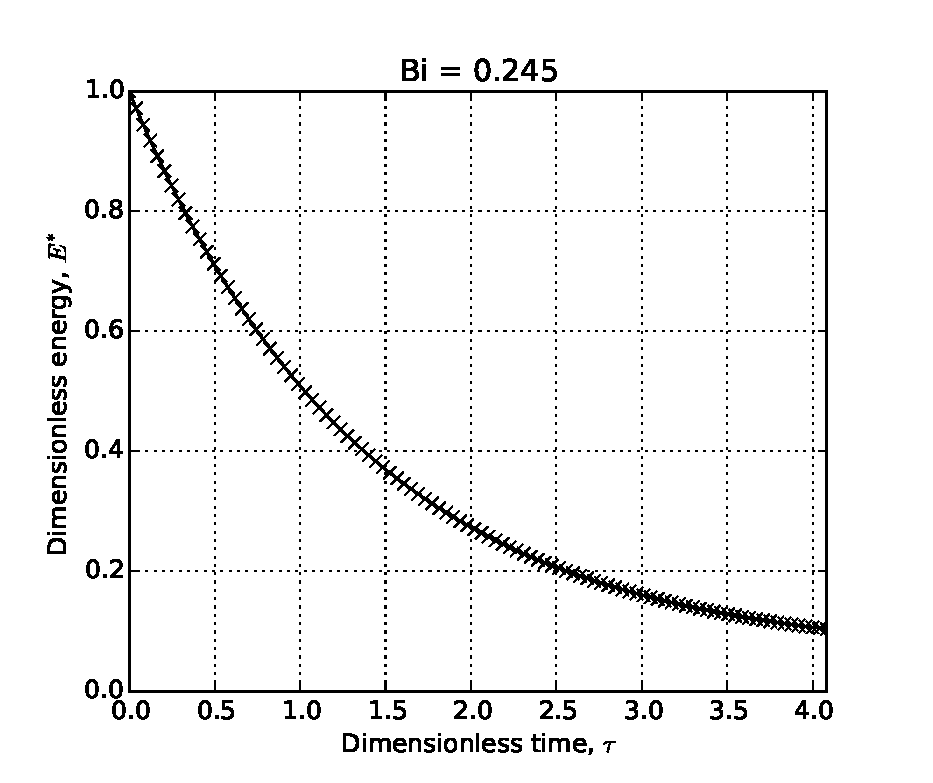
\includegraphics[width=\singleimagewidth]{figures/LC-sphere-in-fluid}
	\caption[Lumped Capacitance energy profile]{Lumped capacitance model: Sphere energy profile decaying from an initial value to a time of $1/\Bi$}
	\label{fig:LC-sphere-in-fluid}
\end{figure}

Reviewing \Cref{eq:theta-lc} we see that the speed of decay is dictated by the term in the exponential, $3\Bi$. Meanwhile, the steady-state value being approached is given by $\frac{G}{3\Bi} = \frac{gR}{h(T_0 - T_f)}$. It is important for this discussion to point out that because both the nondimensional heat generation and Biot number terms contain the solid conductivity, the steady-state value of the lumped capacitance model will not change for varying solid conductivity even if it leads to different Biot numbers.
%~~~~~~~~~~~~~~~~~~~~~~~~~~~~~~~~~~~~~~~~~~~~~~~~~~~~~~~



%~~~~~~~~~~~~~~~~~~~~~~~~~~~~~~~~~~~~~~~~~~~~~~~~~~~~~~~
\subsection{Exact Solution for Sphere}\label{sec:analytic-sphere}

I again analyze the sphere of \Cref{fig:ParticleControlVolume} but now will account for internal temperature gradients inside the sphere. The details of the analytic solution for a sphere with heat generation interacting with a fluid is given in Appendix~\ref{sec:analytic-sphere-details}. Again, solving in terms of the nondimensional temperature and time introduced in \cref{sec:lumped-capacitance} as well as a nondimensional radius,

\begin{align*}
    \theta &= \frac{\mathbb{T}}{\mathbb{T}_0}\\
    \rho & = \frac{r}{R}\\
    \tau & = \frac{t}{R^2/\alpha}
\end{align*}

The energy conservation equation for the sphere with internal temperature gradient, in nondimensional form $\theta_{TG}$, is
\begin{equation}
    \frac{1}{\rho}\frac{\partial^2}{\partial \rho^2}(\rho\theta_{TG}) + G = \frac{\partial\theta_{TG}}{\partial \tau}
\end{equation}

With the initial condition and boundary conditions outlined in \cref{sec:analytic-sphere-details}, the nondimensional temperature distribution inside the sphere is 
\begin{equation}\label{eq:analytic-temperature-distribution}
    \theta_{TG}(\rho,\tau) = \left(\frac{G}{6} + \frac{G}{3\Bi}-\rho^2\right)  +   \sum_{n=1}^\infty \exp(-\zeta^2 \tau) \frac{\sin(\zeta_n \rho)}{\rho} \frac{Z(\zeta_n)}{N(\zeta_n)}  
\end{equation}
where $\zeta_n$ are the eigenvalues of the equation and the functions of $\zeta_n$ ($Z$,$N$,$C$) are given in \cref{sec:analytic-sphere-details}.

The accompanying nondimensional energy of the sphere is integrated to,
\begin{equation}
\label{eq:analytic-energy-profile}
    E^*_{TG}(\tau)=\left(\frac{G}{15}+\frac{G}{3\Bi}\right)+3\sum_{n=1}^\infty \exp(-\zeta^2 \tau) \frac{Z(\zeta_n)}{N(\zeta_n)} C_n(\zeta_n)
\end{equation}

I now compare the exact solution from \Cref{eq:analytic-energy-profile} to the solution of energy given by the lumped capacitance model of \Cref{eq:lc-energy-profile}. The two profiles are given in \Cref{fig:LC-analytic-sphere-in-fluid}. 

\begin{figure}[ht]
	\centering
		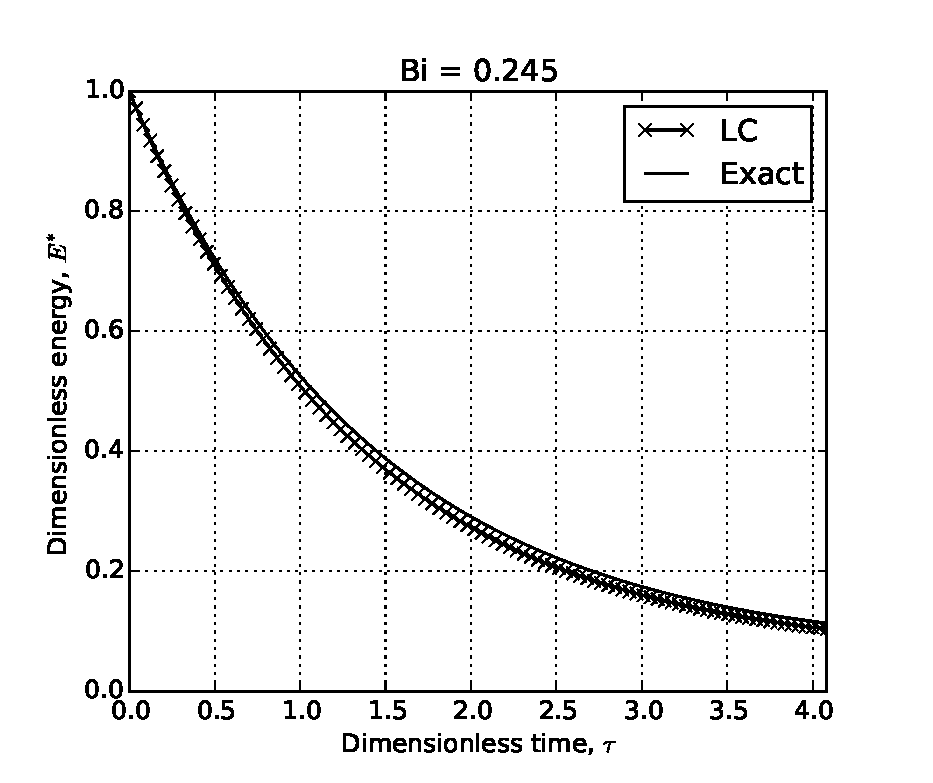
\includegraphics[width=\singleimagewidth]{figures/LC-analytic-sphere-in-fluid}
	\caption[Analytic temperature profile for $\Bi < 1$]{Analytic and lumped capacitance models: Sphere energy profile decaying from an initial value to a time of $1/\Bi$}
	\label{fig:LC-analytic-sphere-in-fluid}
\end{figure}

For the value of Biot number here, $\Bi = 0.245$, the energy profile of the analytic solution of the sphere cooling in a flow is well-captured by the lumped capacitance model. The maximum relative error over the time span, as defined by
\begin{equation}\label{eq:error}
	\text{error} = \frac{\big|E^*_{TG}(\tau) - E^*_{LC}(\tau) \big|}{E^*_{TG}(\tau)}
\end{equation}
is always less than 10\%. 

Consider now the same size sphere but with the Biot number increased by an order from: a) a conductivity of $k = k_r/10$ and b) a heat transfer coefficient of $h = 10h_f$. The two physical changes to the system result in the same Biot number ($\Bi = 2.45$) but as we can see in \Cref{fig:LC-analytic-sphere-in-fluid-Bi-2}, there are drastic differences between the energy profiles.

\begin{figure}
        \centering
        \begin{subfigure}[b]{0.5\textwidth}
                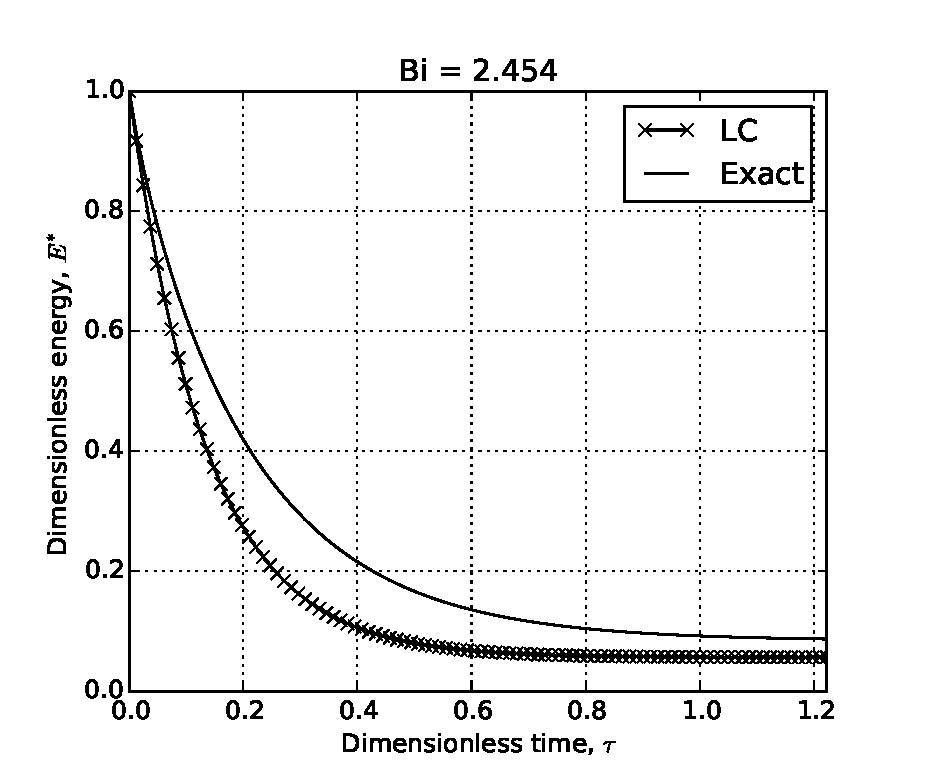
\includegraphics[width=\textwidth]{figures/LC-analytic-sphere-in-fluid-Bi-2a}
                \caption{$k \uparrow$, lumped capacitance error in the transient and steady-state.}
				\label{fig:LC-analytic-sphere-in-fluid-Bi-2a}
        \end{subfigure}%
        
          %add desired spacing between images, e. g. ~, \quad, \qquad, \hfill etc.
          %(or a blank line to force the subfigure onto a new line)
        \begin{subfigure}[b]{0.5\textwidth}
                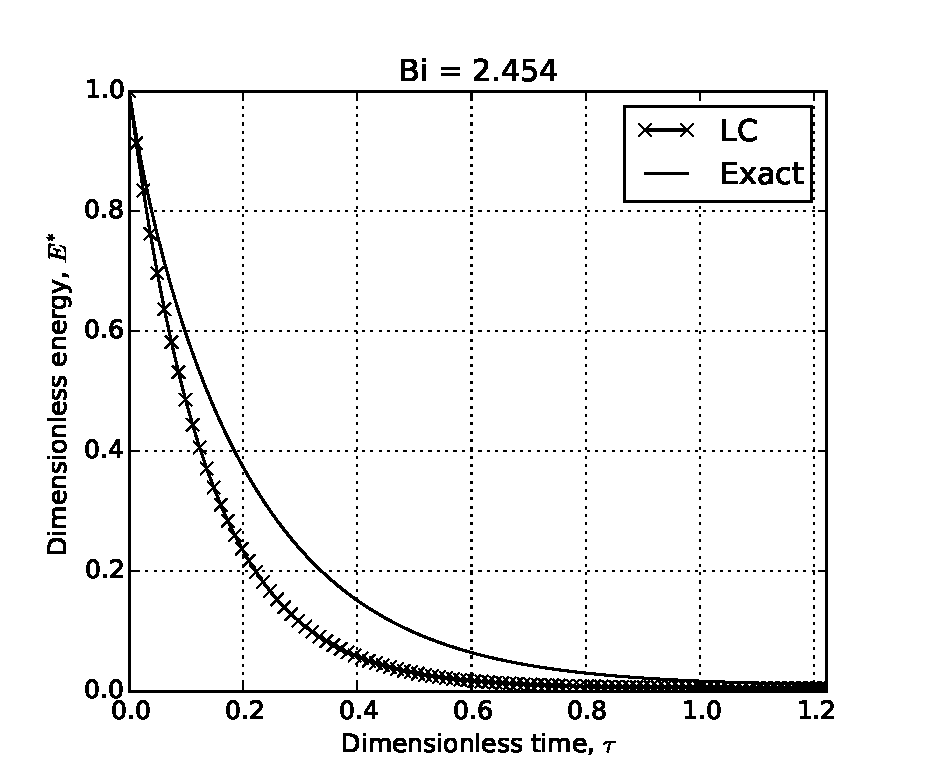
\includegraphics[width=\textwidth]{figures/LC-analytic-sphere-in-fluid-Bi-2b}
                \caption{$h \uparrow$, lumped capacitance error mainly in the transient.}
				\label{fig:LC-analytic-sphere-in-fluid-Bi-2b}
        \end{subfigure}
        \caption[Analytic temperature profile for moderate Biot number]{Analytic and lumped capacitance models: Sphere energy profile decaying from an initial value to a time of $3/\Bi$. The same Biot number produces different results for the exact solution of a sphere with heat generation.}\label{fig:LC-analytic-sphere-in-fluid-Bi-2}
\end{figure}

Seen in \Cref{fig:LC-analytic-sphere-in-fluid-Bi-2a}, the lumped capacitance solution both over-predicts the speed at which the sphere reaches a thermal steady-state as well as the value of the steady-state. Comparatively, in \Cref{fig:LC-analytic-sphere-in-fluid-Bi-2b}, for the same Biot number, the lumped capacitance solution again over-predicts the speed to thermal steady-state by the same rate but is relatively accurate for the steady-state value itself. 

Viewing the steady-state terms of the two solutions, the source of the error becomes apparent. From \Cref{eq:analytic-energy-profile}, the steady-state term of the exact solution is
\begin{equation}
	E^*_{TG,ss}=\frac{G}{15}+\frac{G}{3\Bi}
\end{equation}

Whereas, the steady-state term of the lumped capacitance solution from \Cref{eq:lc-energy-profile} is,
\begin{equation}
	E^*_{LG,ss} = \frac{G}{3\Bi}
\end{equation}

The two steady-state values differ only by the additional term of $\frac{G}{15}$ on the exact solution. This term appears in the exact solution from integration of the temperature gradient that exists in the pebble due to volumetric heating (see \cref{sec:analytic-sphere-details}). The lumped capacitance solution assumes no internal temperature gradient in the sphere and thus by definition can not account for this $\frac{G}{15}$ term. Furthermore, the nondimensional heat generation term, $G$, given in \Cref{eq:nondimensional-heat-generation}, is importantly a function of thermal conductivity but not the heat transfer coefficient. The lack of dependence on $h$ explains the difference between steady-state values in \Cref{fig:LC-analytic-sphere-in-fluid-Bi-2}  When $\Bi$ is small, the steady state error between lumped capacitance and the exact solution is small. If only $h$ increases the error in steady-state remains small. This is demonstrated in \Cref{fig:LC-analytic-sphere-in-fluid-Bi-2b} when steady-state solutions are close. However, in \Cref{fig:LC-analytic-sphere-in-fluid-Bi-2a} as $k$ was reduced, the curves no longer converge to similar steady-states. This phenomena appears only with the combination of low conductivity materials with volumetric heating.

Even in cases without volumetric heating, when the Biot number grows large, errors appear in the transient portion of curves but ultimately converge to the same steady-state solutions. To address the inaccuracies in the time-dependent response of the lumped capacitance method with large Biot number, a correction factor, implemented by Van Lew and Xu\etal~in situations without heat generation, is employed.\cite{VanLew2010,Xu2012}. In their work, they considered a heat transfer fluid interacting with a low conductivity thermal storage material. The solar thermal storage systems they analyzed often had moderate-to-large Biot numbers but they could continue to apply the lumped capacitance model in their calculations with application of a so-called Jeffreson Correction.\cite{jeffreson409} However, because their applications did not involve heat generation, its usefulness for application in our pebble beds absorbing nuclear heat is validated.
%~~~~~~~~~~~~~~~~~~~~~~~~~~~~~~~~~~~~~~~~~~~~~~~~~~~~~~~





%~~~~~~~~~~~~~~~~~~~~~~~~~~~~~~~~~~~~~~~~~~~~~~~~~~~~~~~
\subsection{Jeffreson Correction for Sphere with Nuclear Heating}
The correlation to correct the heat transfer coefficient due to solids with large Biot number is given by Jeffreson as,\cite{jeffreson409}
\begin{equation}
	h_{p}=\frac{h}{1+\Bi/5}
\end{equation}
where $h_p$ is the modified heat transfer coefficient of the particle with an internal temperature gradient. As the Biot number increases, the modified heat transfer coefficient decreases. THe form of this correlation works to effectively slow down the rate of heat removed by the passing fluid. Recall the curves of Fig~\ref{fig:LC-analytic-sphere-in-fluid-Bi-2}. where the lumped capacitance solution over-predicted the speed with which the energy decayed towards steady-state. A modified Biot number can then also be written as
\begin{equation}\label{eq:jeffreson-correction-bip}
	\Bi_p = \frac{h_p d}{k_r} = \frac{\Bi}{1+\Bi/5}
\end{equation}

Applying the Jeffreson Correction to \Cref{eq:theta-lc}, the modified lumped capacitance solution is written now in terms of the modified Biot number,
\begin{equation}
\label{eq:theta-jc-bip}
	\theta_{JC}=\left(1-\frac{G}{3\Bi_p}\right)\exp\left(-3\Bi_p \tau\right) + \frac{G}{3\Bi_p}
\end{equation}
and thereby \Cref{eq:lc-energy-profile} also yields
\begin{equation}\label{eq:jc-energy-profile}
	E^*_{JC}(\tau) = \left(1-\frac{G}{3\Bi_p}\right)\exp\left(-3\Bi_p \tau\right) + \frac{G}{3\Bi_p}
\end{equation}

The energy profiles from the lumped capacitance model (LC), the Jeffreson correction (JC), and the exact solution are all plotted together in \Cref{fig:LC-JC-analytic-sphere-in-fluid-Bi-2}. Barely visible under the JC solution are teh curves from the exact solution. The Jeffreson correction to the lumped capacitance method allows the simple modeling approach of the lumped capacitance method to capture the proper transient as well as steady-state values for this sphere with a moderately sized Biot number. 

\begin{figure}
        \centering
        \begin{subfigure}[b]{0.5\textwidth}
                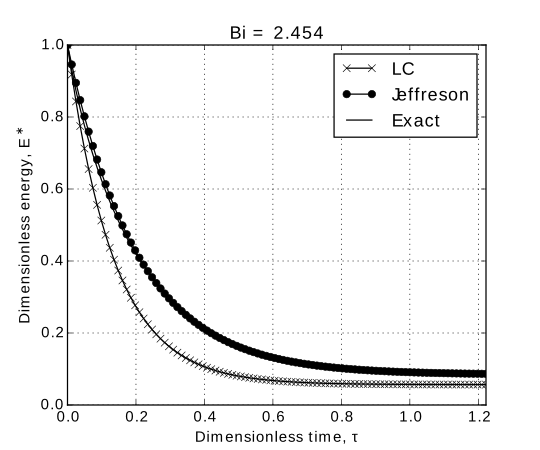
\includegraphics[width=\textwidth]{figures/LC-JC-analytic-sphere-in-fluid-Bi-2a}
                \caption{The Biot number increased from a decrease in the solid conductivity.}
				\label{fig:LC-JC-analytic-sphere-in-fluid-Bi-2a}
        \end{subfigure}%
        
          %add desired spacing between images, e. g. ~, \quad, \qquad, \hfill etc.
          %(or a blank line to force the subfigure onto a new line)
        \begin{subfigure}[b]{0.5\textwidth}
                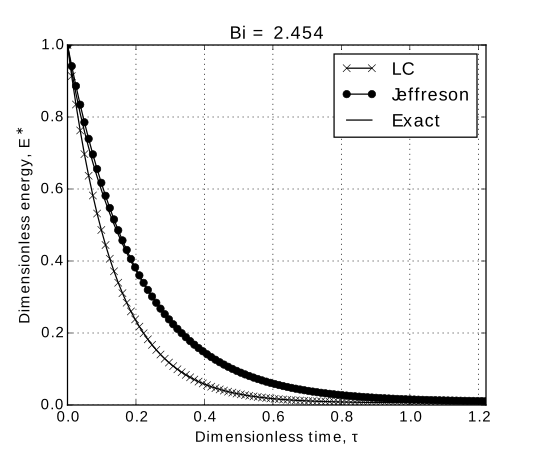
\includegraphics[width=\textwidth]{figures/LC-JC-analytic-sphere-in-fluid-Bi-2b}
                \caption{The Biot number increased from  an increase in the heat transfer coefficient.}
				\label{fig:LC-JC-analytic-sphere-in-fluid-Bi-2b}
        \end{subfigure}
        \caption[Jeffreson correction for moderate Biot number based on conductivity]{Analytic, lumped capacitance model, and LC model with Jeffreson correction: Jeffreson correction corrects for transient and steady-state errors of lumped capacitance.}\label{fig:LC-JC-analytic-sphere-in-fluid-Bi-2}
\end{figure}

\begin{figure}
        \centering
        \begin{subfigure}[b]{0.5\textwidth}
                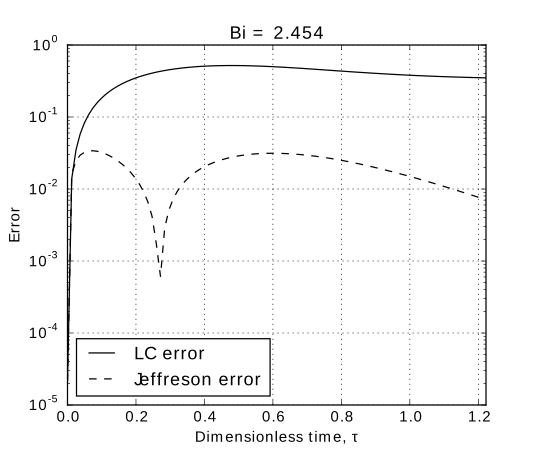
\includegraphics[width=\textwidth]{figures/LC-JC-analytic-error-Bi-2a}
                \caption{The Biot number increased from a decrease in the solid conductivity.}
				\label{fig:LC-JC-analytic-error-Bi-2a}
        \end{subfigure}%
        
          %add desired spacing between images, e. g. ~, \quad, \qquad, \hfill etc.
          %(or a blank line to force the subfigure onto a new line)
        \begin{subfigure}[b]{0.5\textwidth}
                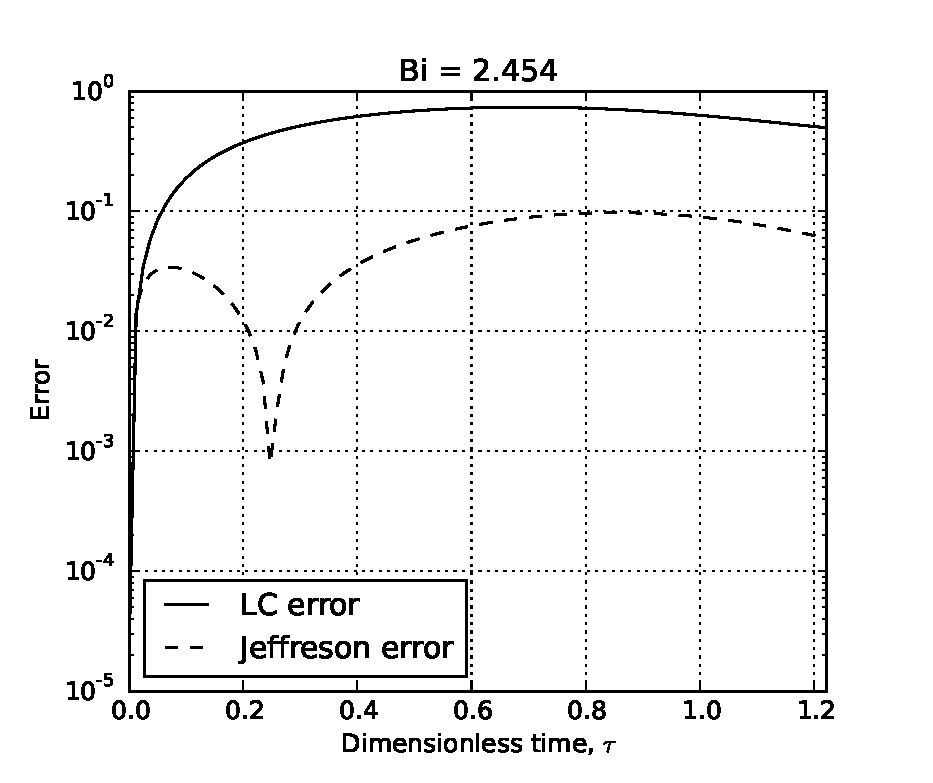
\includegraphics[width=\textwidth]{figures/LC-JC-analytic-error-Bi-2b}
                \caption{The Biot number increased from  an increase in the heat transfer coefficient.}
				\label{fig:LC-JC-analytic-error-Bi-2b}
        \end{subfigure}
        \caption[Error of lumped capacitance and Jeffreson correction for moderate Biot number]{Error of lumped capacitance and reduced error of the model with Jeffreson correction for moderate Biot number.}\label{fig:LC-JC-analytic-error-Bi-2}
\end{figure}

To look more closely, we view the instantaneous error (see \Cref{eq:error}) in \Cref{fig:LC-JC-analytic-error-Bi-2}. For the value of $\Bi > 1$ due to either low conductivity (\Cref{fig:LC-JC-analytic-error-Bi-2a}) or high heat transfer coefficient (\Cref{fig:LC-JC-analytic-error-Bi-2b}), the error in the Jeffreson correction is always under 10\%; often closer to only 1\%. This is in opposition to the standard lumped capacitance method which has 50-80\% error for both transient and steady-state values.

The lumped capacitance method allows researchers to simplify transient, conjugate heat transfer problems to a situation with an isothermal solid. In the discrete element method, the assumption of isothermal solid is innate in the framework of the method. With the implementation of the Jeffreson correction in the discrete element method, we have confidence in the fidelity of the heat transfer with the helium flow for moderately sized Biot numbers. The Jeffreson correction will be implemented into the DEM computations \textit{via} \Cref{eq:jeffreson-correction-bip}. 
%~~~~~~~~~~~~~~~~~~~~~~~~~~~~~~~~~~~~~~~~~~~~~~~~~~~~~~~







\FloatBarrier
\section{Benchmarking Solid-solid and Solid-fluid Heat Transfer Models for Pebble Beds}\label{sec:cfd-validate}

\subsection{Validating Pressure Drop in Packed Beds with Flowing Helium Purge Gas}
Our three-dimensional system consists of mono-dispersed particles of diameter $d_p$. The particles are constrained by two rigid walls in the $x$-direction at locations of $x = \pm 10d_p$  and periodic boundary conditions in the $y$-direction located at $y = \pm 7.5d_p$. Gravity acts in the downward $z$-direction and the particles are bound from below by a rigid wall at $z=0$. The size of the system allows approximately \num{10000} particles to fill to a height of approximately $z = 30d_p$. The volume was chosen to represent the long, tall, narrow channels seen in many solid breeder module designs\cite{Cho2008,Poitevin2010,Enoeda2003}. The fluid domain is constructed to include an inlet and outlet region of fluid to permit development of the flow profiles. The inlet region is 5 pebble diameters in length and the outlet is 30 pebble diameters. No-slip boundary conditions are enforced at the walls at the $x$-limits of the region. To match the DEM domain, periodic boundary conditions are used in the $y$-limits. The inlet face of the fluid is specified at a constant $\vec{v} = (5, 0, 0)$ \si{\centi\meter\per\second}. The outlet face is specified with OpenFOAM's `inletOutlet' command with a given pressure. This boundary condition allows the inlet pressure to float to value that satisfies the specified inlet velocity and outlet pressure. 

The size of the CFD cells were chosen to be large enough to fit approximately 5 pebbles, for which the divided technique of computing void fraction is applicable (see \cref{sec:lag-eul-mapping}); the ratio of cell volume to particle volume was $V_\text{cell} / V_p = 7.46$. The helium, for this first validation, was modeled with constant fluid properties. The values are given in Table~\ref{tab:cfd-properties}.

The Koch-Hill-Ladd drag model is employed in the style of Model B with an Archimedes pressure for buoyancy term. The terminology of these CFD coupling drag models is discussed in Ref.~\cite{Zhou2010} The Nusselt number correlation of Li \& Mason is used for calculating the Nusselt number. OpenFOAM's dummy turbulence model (which is nothing more than a laminar model) is used.

An implicit time marching scheme is employed with a time step in the fluid domain of $\Delta t_f =$\SI{1e-4}{\second}. The small time step is not necessary to capture the fluid flow. The momentum equation is essentially not even transient as a steady-state laminar solution is achieved almost instantaneously in comparison to the long time span required to reach thermal steady state. The small time step is necessary for a relatively tight coupling to the pebble bed as the temperatures increase on the pebbles. Integration schemes of gradients, divergence terms, and laplacians are all Gauss linear or Gauss limitedLinear (as defined in OpenFOAM). The time step of the DEM is $\Delta t_s =$ \SI{1e-7}{\second} which must be small for stability of the DEM explicit integration. The coupling between CFD and DEM domains occurs every 10 time steps of the fluid domain - equating to every \num{10000} in the pebble domain.

The layout of the pebble bed inside the CFD domain is shown in \Cref{fig:cfdem-domain-y,fig:cfdem-domain-z}. Notable of the layout is the relaxation of the mesh size in the direction of the periodic boundaries. The size is permitted as there are few variations in fluid or temperature in the periodic direction. The meshes are made much smaller in the direction between cooling boundaries. In this direction ($x$-direction), we need the meshes small enough to resolve a temperature and velocity profiles across the bed between centerline and cooling boundaries. We also want to capture the behavior of near-wall arrangement of the pebble bed. 

\begin {table}[htp] %
\caption{Constant fluid properties of helium purge gas in CFD-DEM coupling.}
\label {tab:cfd-properties} \centering %
\begin {tabular}{ ccccc }
\toprule %
$\nu$				&	$\alpha$				&	$k$		&	$C_p$		& $\rho$		\\
(\si{\meter\squared\per\second})			&	(\si{\meter\squared\per\second})				&	(\si{\watt\per\meter\per\kelvin})	&	(\si{\joule\per\kilogram\per\kelvin})	& (\si{\kilogram\per\cubic\meter})	\\\toprule
\num{4.02e-4} &	\num{6.06e-4}	& 	\num{0.2}		& 	\num{5192.8}		& 	\num{0.175}		\\\bottomrule
\end{tabular}
\end{table}


% \begin{figure}[t]
% 	\centering
% 	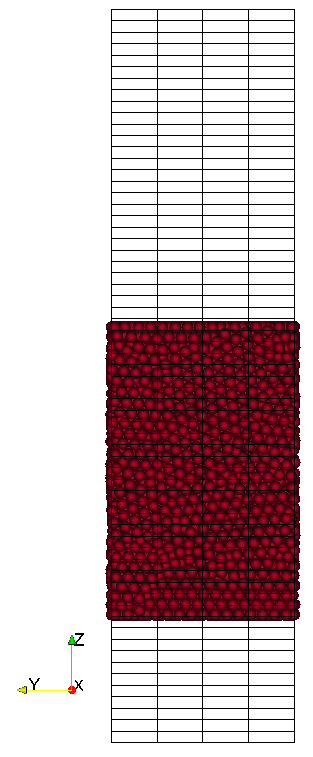
\includegraphics[width=0.4\textwidth]{figures/x-side-view}
%     \caption{Side view of the pebble bed as it resides in the CFD mesh. The meshes in the direction of the periodic faces are allowed to be larger than others.}\label{fig:cfdem-domain-x}
% \end{figure}

\begin{figure}[t]
	\centering
	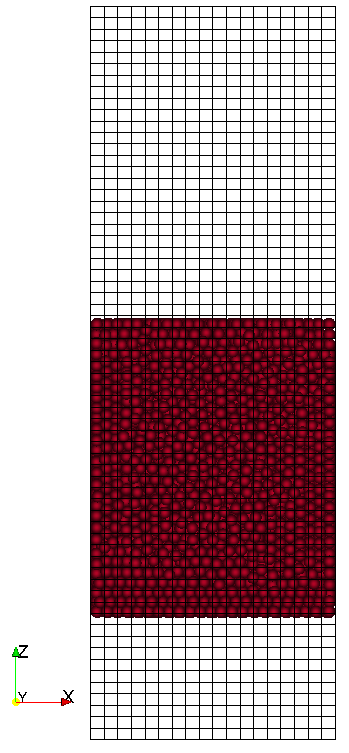
\includegraphics[width=0.4\textwidth]{figures/y-side-view}
    \caption{Front view of the pebble bed as it resides in the CFD mesh. The meshes in the direction of cooling are chosen to be large enough to fit many pebbles but small enough to provide a resolved temperature profile.}\label{fig:cfdem-domain-y}
\end{figure}

\begin{figure}[t]
	\centering
	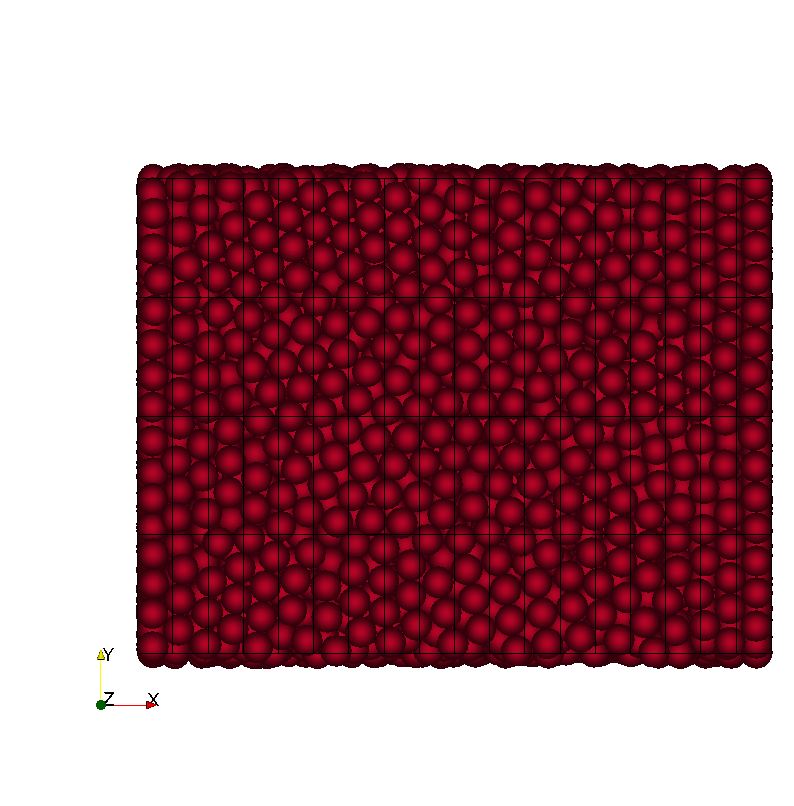
\includegraphics[width=\singleimagewidth]{figures/z-top-view}
    \caption{Top view of the pebble bed as it resides in the CFD mesh.}\label{fig:cfdem-domain-z}
\end{figure}


The CFD-DEM model was run at various particle Reynolds numbers and the overall pressure drop of the packed bed was measured. The pressure drop is compared against the well-known Kozeny-Carman and Ergun equations. The Kozeny-Carman is known to fit better with experimental data at very small Reynolds numbers while the Ergun equation is a more general equation meant to span a large range of Reynolds numbers. In \Cref{fig:cfdem-pressure-drop} we see the CFD-DEM coupling model is providing bed-scale pressure drops that match very well with Kozeny-Carman over the Reynold’s numbers applicable to helium purge flow in fusion reactors ($\Re_p \approx 1$). 

Seki\etal~experimentally studied the flow of helium purge gas in efforts to better understand tritium recovery.\cite{Seki2013} They ran a representative volume of pebbles up to flow rates of \SI{100}{\liter\per\minute} and also found that Ergun's pressure drop prediction was highly accurate for the pebble beds as long as the viscous contribution (see the right-most term in \Cref{eq:ergun-pressure}) was small, \textit{e.g.} when the Reynolds number of the packed bed is small. This result is a strong validation of the macroscopic results of pressure drop as calculated by the CFD-DEM simulation of a packed bed.

\begin{figure}
\centering
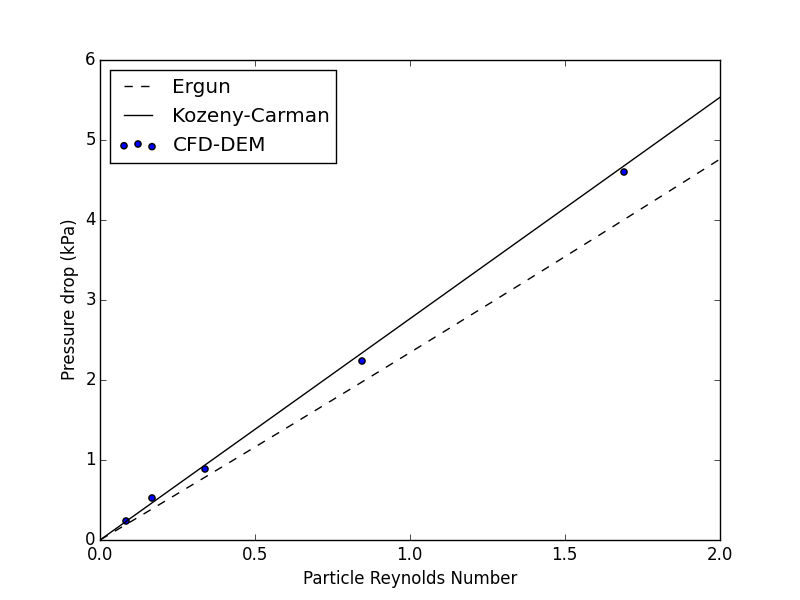
\includegraphics[width=.7\textwidth]{figures/pressureDrops-full.png}
\caption{Pressure drop calculations across packed beds, solved by CFD-DEM, fit well to the Kozeny-Carman empirical relation.}\label{fig:cfdem-pressure-drop}
\end{figure}


\FloatBarrier
\subsection{Effective Thermal Conductivity from CFD-DEM with Stagnant Helium}\label{sec:cfd-dem-effective-conductivity}
In \Cref{sec:dem-benchmark} we saw that DEM models, including contact roughness modeling, were able to effectively model heat transfer of pebble beds in vacuum by means of measuring effective thermal conductivity of a representative pebble bed. We consider the same pebble bed but now immerse the pebbles in a stagnant helium gas. The fluid volume surrounding the pebble bed has equal dimensions in the $x$- and $y$-directions. A constant length $50d_p$ was used in the $z$-direction. The boundaries were: periodic in $y$, adiabatic in $z$, and constant temperature, $T_w = \SI{573}{\kelvin}$ in $x$. A constant nuclear heating rate of $q_p'''=\SI{8}{\mega\watt\per\cubic\meter}$ was applied to the pebble volumes. The simulation is allowed to run to thermal steady-state. 

After reaching a steady solution, temperature distributions of the pebbles are used to calculate an effective thermal conductivity. For the first set of pebble beds, the Jeffreson correction is not applied. The temperature distribution is given in \Cref{fig:keff-cfd-initial}. 

\begin{figure}[!ht]
    \centering
    \begin{subfigure}[b]{0.45\textwidth}
        \centering
        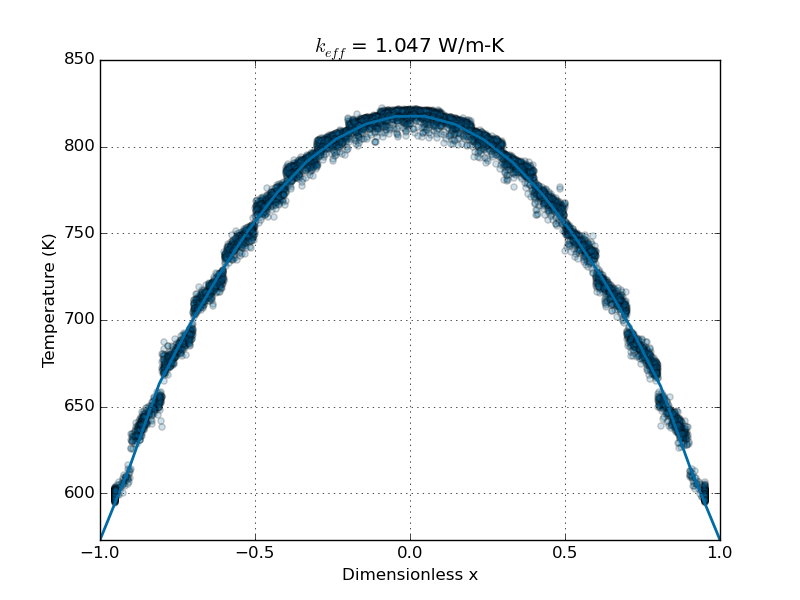
\includegraphics[width=\textwidth]{figures/initial_packing_study/keff-cfd-62.png}
        \caption{$\phi_i = 62\%$}
    \end{subfigure}
    ~
    \begin{subfigure}[b]{0.45\textwidth}
        \centering
        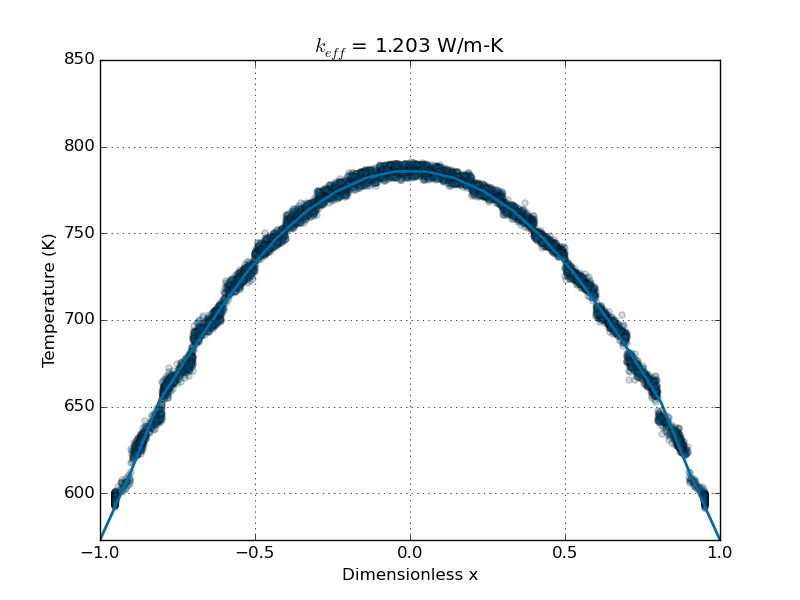
\includegraphics[width=\textwidth]{figures/initial_packing_study/keff-cfd-64.png}
        \caption{$\phi_i = 64\%$}
    \end{subfigure}
    \caption{$\keff$ for packed beds in stagnant helium.}
\label{fig:keff-cfd-initial}
\end{figure}

In addition, a grid-independence study was run. The grid size was reduced by 50\% in each case and $\keff$ was calculated. The results for each grid are given in \Cref{fig:cfd-grid-study}. Negligible change was found between the two finer cases and consequently the results given here are of the finest mesh.

\begin{figure}[ht]
\centering
    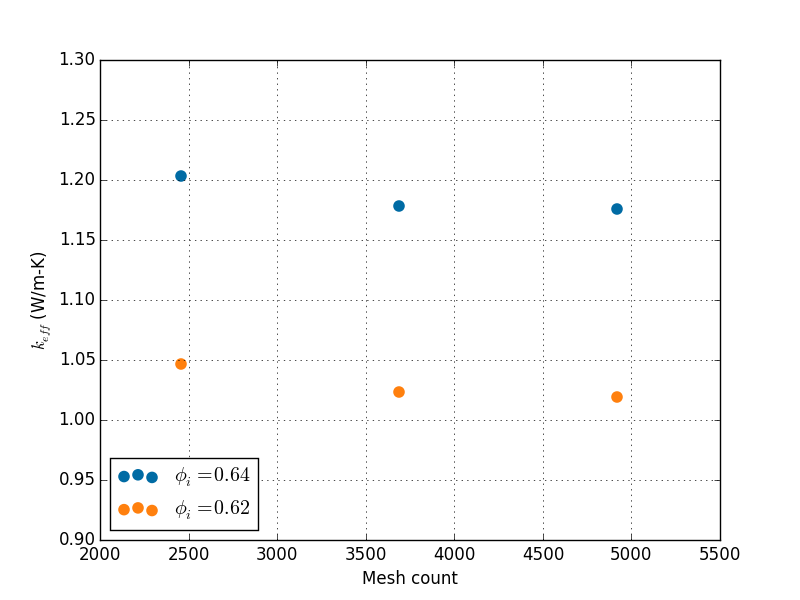
\includegraphics[width=\singleimagewidth]{figures/cfd-grid-study.png}
    \caption{Effective thermal conductivity as a function of the grid size. The change between $\keff$ becomes negligible at the finer grid sizes.}
    \label{fig:cfd-grid-study}
\end{figure}

For stagnant helium, the Nusselt number is $\Nu = 2$ which leads to a heat transfer coefficient of
\begin{equation}
h = \frac{k_f\Nu}{d_p}
\end{equation}
where $k_f$ is the thermal conductivity of helium, $k_f =\SI{0.34}{\watt\per\meter\per\kelvin}$. The heat transfer coefficient is therefore $h = \SI{680}{\watt\per\meter\squared\per\kelvin}$

The Biot number, using solid conductivity of $k_s =\SI{2.4}{\watt\per\meter\per\kelvin}$, is
\begin{equation}
\Bi = \frac{h d_p}{k_s} = 0.283
\end{equation}
which is small enough that the Biot assumption should not be highly inaccurate. Nevertheless, a second set of pebble beds is run with Jeffreson correction applied. The corrected heat transfer coefficient is reduced to
\begin{equation}
h' = \frac{\SI{680}{\watt\per\meter\squared\per\kelvin}}{1 + 0.283/5} = \SI{643}{\watt\per\meter\squared\per\kelvin}
\end{equation}
which results in a 5\% drop in heat transfer coefficient with the Jeffreson correction applied.
Using the Jeffreson-corrected heat transfer coefficient for simulations, temperature profiles at thermal steady state are given in \Cref{fig:keff-cfd-initial-jeffreson}. For the case of stagnant helium, the Jeffreson correction had negligible effect on determinations of temperature distributions in the two packed beds studied. 

\begin{figure}[!ht]
    \centering
    \begin{subfigure}[b]{0.45\textwidth}
        \centering
        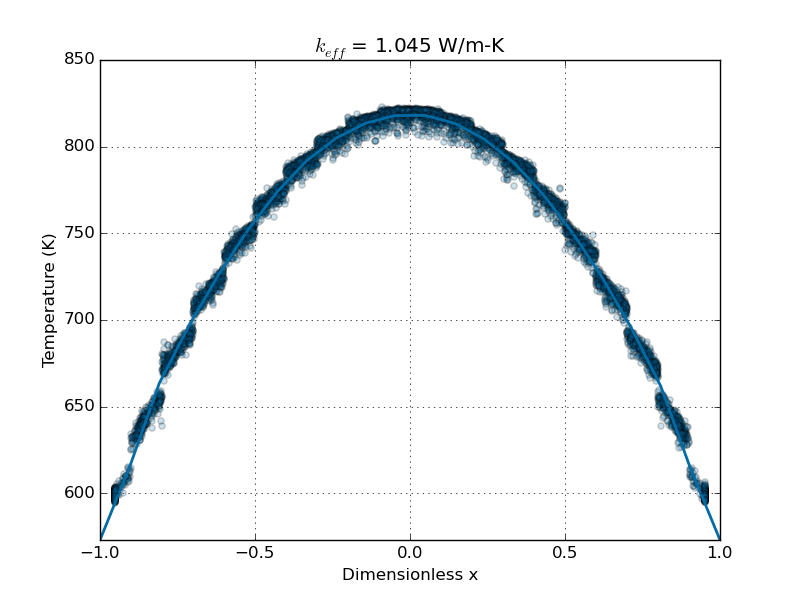
\includegraphics[width=\textwidth]{figures/initial_packing_study/keff-cfd-jeffreson-62.png}
        \caption{$\phi_i = 62\%$}
    \end{subfigure}
    ~
    \begin{subfigure}[b]{0.45\textwidth}
        \centering
        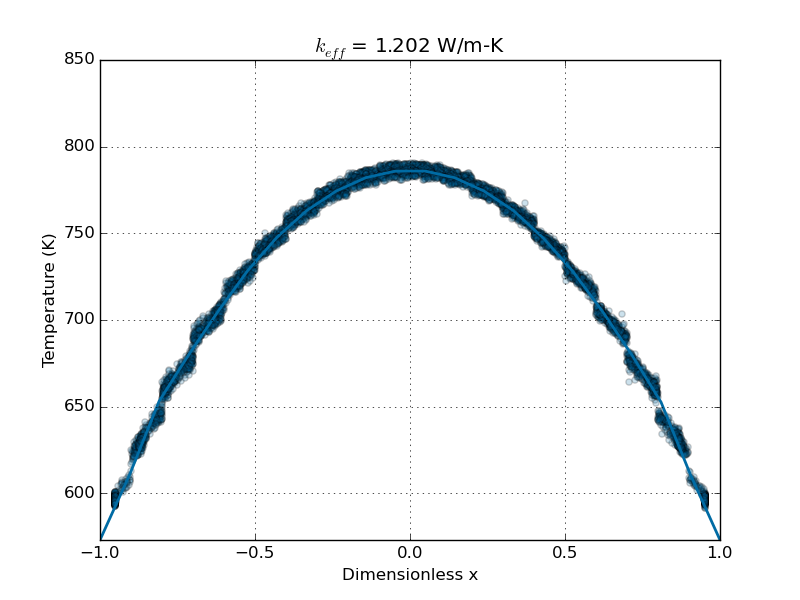
\includegraphics[width=\textwidth]{figures/initial_packing_study/keff-cfd-jeffreson-64.png}
        \caption{$\phi_i = 64\%$}
    \end{subfigure}
    \caption{$\keff$ for packed beds in stagnant helium with Jeffreson correction to heat transfer coefficient.}
\label{fig:keff-cfd-initial-jeffreson}
\end{figure}

\FloatBarrier

Comparing the results of pebble beds with Jeffreson correction applied, for a stagnant fluid with $\Nu = 2$, with material producing $\Bi = 0.29$, there is a negligible change to the effective thermal conductivity of beds without the correction. Nevertheless, the correction is costs practically no computational time and is trivially applied during the convection calculation routine in the code. For cases when the Nusselt number increases locally, the effect may be larger and is therefore applied in general to CFD-DEM coupling code.

In the current framework, constant thermal properties are implemented for helium gas. The transport properties used in this study were from averages between \SI{300}{\celsius} and \SI{900}{\celsius}, a range over which the properties were all fairly linear. This is equivalent to reporting data at an average bed temperature of \SI{600}{\celsius}. Hatano\etal~reported the effective thermal conductivity of \lit~was reported for a packed bed of $d_p = \SI{1.91}{\milli\meter}$ as approximately $\keff =\SI{1.18}{\watt\per\meter\per\kelvin}$ with the hot-wire technique.\cite{Hatano2003} Tanigawa\etal~reported the effective thermal conductivity at \SI{600}{\celsius} as a function of compressive strain and series cycle.\cite{Tanigawa2005801} The results of Tanigawa\etal~are reproduced in \Cref{fig:tanigawa}; the values are approximately $\keff =\SI{1.3}{\watt\per\meter\per\kelvin}$ above a stress state on the bed of \SI{1}{\mega\pascal}. Abou-Sena\etal~measured the effective thermal conductivity of uncompressed \lit~but only up to temperatures of \SI{500}{\celsius}, and are therefore not relevant to comparison here.\cite{Abou-Sena:2007ff} Mandal\etal~measured the effective thermal conductivity of \lit~pebbles in stagnant and flowing helium environment.\cite{Mandal2012} However, the results of Mandal\etal~are much lower than data from other members, they report $\keff =\SI{0.274}{\watt\per\meter\per\kelvin}$ in a stagnant helium environment at \SI{200}{\celsius} which is 20\% of values of other research centers. At their lowest superficial velocity, $u_s = \SI{0.146}{\meter\per\second}$, they find an effective conductivity of $\keff = \SI{0.65}{\watt\per\meter\per\kelvin}$ with $d_p = \SI{1}{\milli\meter}$ pebbles.

\begin{figure}[ht]
\centering
    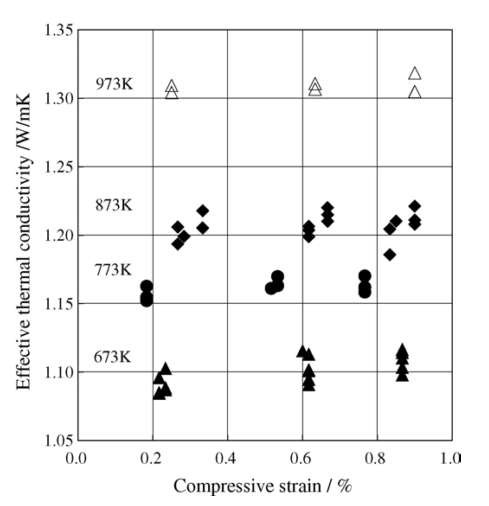
\includegraphics[width=\singleimagewidth]{figures/tanigawa.png}
    \caption{Effective thermal conductivity of a compressed \lit~pebble bed. Reproduced from \cite{Tanigawa2005801}.}
    \label{fig:tanigawa}
\end{figure}

The results found here are in agreement with reported values from literature of uncompressed pebble beds at similar temperatures;\cite{Hatano2003} we found $\keff =\SI{1.05}{\watt\per\meter\per\kelvin}$ when the initial packing fraction was $\phi_i = 0.62$. As the contact forces increased between the pebbles as is the case for initial packing of $\phi_i = 0.64$, we found $\keff =\SI{1.2}{\watt\per\meter\per\kelvin}$. The results of this validation are plotted alongside experimental data in \Cref{fig:keff-cfd-comparisons}.


\begin{figure}[ht]
\centering
    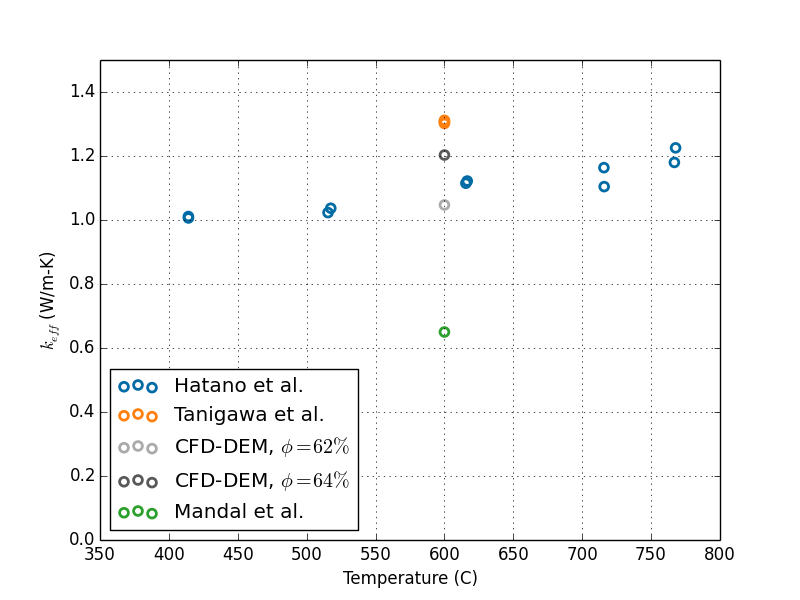
\includegraphics[width=\singleimagewidth]{figures/initial_packing_study/keff-he-comparisons.png}
    \caption{Comparison of effective conductivity measurements for \lit.}
    \label{fig:keff-cfd-comparisons}
\end{figure}


Another important observation to be made from the pebble temperatures of CFD-DEM simulations is the lack of `hot rattlers' that appeared in DEM simulations. For example, in \Cref{fig:keff-rough-initial}, there are many pebbles with temperatures much higher than the majority of nearby pebbles. These pebbles exist in localized pockets where their neighbors are carrying more contact force and they sit with relatively small forces at all contacts. The isolation allows nuclear heating to run away without temperature moderation. Including helium convection on pebble beds resulted in the complete disappearance of all hot rattlers. In \Cref{fig:keff-cfd-initial-jeffreson}, all temperatures in a given region are tightly grouped around average temperatures. This demonstrates that the helium purge gas, while not intended to be a major carrier of heat in the system, plays a role in thermally equilibrating temperatures between pebbles and moderating temperatures of any mechanically isolated pebbles. This also has implications for fragmentation in pebble beds with helium. Small fragments were seen in \Cref{sec:failure-study} to travel through beds before coming to rest with very small contact forces. We will see in \Cref{sec:dem-studies} that helium moderates fragmentation temperatures just as it did hot rattlers.











\FloatBarrier



%%%%%%%%%%%%%%%%%%%%%%%%%%%%%%%%%%%%%%%%%%%%%%%%%%%%%%%%%%%%%%%%%%%%%%%%%%%%%%%%%%%%%%%%%%%%%%%%%%%%%%%%%%%%
%%%%%%%%%%%%%%%%%%%%%%%%%%%%%%%%%%%%%%%%%%%%%%%%%%%%%%%%%%%%%%%%%%%%%%%%%%%%%%%%%%%%%%%%%%%%%%%%%%%%%%%%%%%%
%
% new section
%
%%%%%%%%%%%%%%%%%%%%%%%%%%%%%%%%%%%%%%%%%%%%%%%%%%%%%%%%%%%%%%%%%%%%%%%%%%%%%%%%%%%%%%%%%%%%%%%%%%%%%%%%%%%%
%%%%%%%%%%%%%%%%%%%%%%%%%%%%%%%%%%%%%%%%%%%%%%%%%%%%%%%%%%%%%%%%%%%%%%%%%%%%%%%%%%%%%%%%%%%%%%%%%%%%%%%%%%%%
\section{Summary of CFD-DEM Modeling of Solid Breeder Pebble Beds}
The physics of heat transfer in solid breeder pebble beds are innately multi-scale. On one hand, heat transfer through contact conductance is strongly dependent on the contact force network established in the packed bed of solids. During operation of the solid breeder in a fusion reactor, the force network and packing structure are bound to evolve due to, for example, forces on pebbles and fragmentation of individual pebbles. The impact on heat transfer due to pebble-scale interactions is important to capture with numerical models because of the narrow operating temperature imposed on solid breeders. On the other hand, the slow-moving helium purge gas is a larger-scale interaction as the fluid transports heat well beyond the range of individual pebbles. Experimentally, helium's contribution to effective thermal conductivity has long been known to be larger than solid conductance and is critical to models of temperature distributions of solid breeder pebble beds.

Likewise, we use a multi-scale approach to heat transfer modeling of the pebble beds. Lithium ceramic pebbles are handled with the DEM code introduced in \Cref{ch:modeling-development}. DEM models allow continual monitoring of inter-particle forces and individual particle temperatures such that any of the crush-prediction, fragmentation, or thermal expansion methods allow modeling changes of packing structures. Helium is treated with a continuum approach using volume-averaged versions of conservation equations of Navier-Stokes and energy. The volume-averaged approach of the fluid allow for an efficient overlaying of the fluid contribution to the thermophysical behavior of the pebble bed. Closure of coupled fluid conservation equations is easily performed \textit{via} summed contributions of particles in fluid computational space. 

We tested the validity of the lumped capacitance assumption when pebbles experience heat generation with a moderately large Biot number. Inaccuracies appeared for calculations of both transient and steady-state temperatures in a single pebble, with heat generation, when immersed in a passing fluid. The inaccuracies were larger for cases when solid conductivity decreased compared to cases when heat transfer coefficient increased -- even if the two cases had the same Biot number. This was shown to be an effect of heat generation internal to the solid and standard lumped-capacitance validity on Biot number was invalidated. However, by incorporating the Jeffreson correction to heat transfer coefficients, we showed lumped-capacitance approximations (with Jeffreson correction) continues to be accurate even under the condition of volumetric heating of the solid. The Jeffreson correction is implemented in the CFD-DEM solver for solid breeder pebble beds.

A benchmarking effort was made to validate the application of this CFD-DEM model for the specific conditions of solid breeder packed beds. A parametric study of Reynolds number showed that the coupled codes were able to recreate the pressure drop predicted by Kozeny-Carman correlation. From the point of view of heat transfer, CFD-DEM models of heat transfer in a stagnant helium bed were compared to experimental measurements of \lit~pebble beds and seen to be in sufficient agreement, considering the assumptions made for the computational models.

The CFD-DEM model is a powerful and efficient means of simulating helium flow through packed beds, while retaining heat transfer contributions of pebbles and their packing structure. However the simplicity of the volume-averaging model sacrifices the ability to resolve the complex flow fields that develop in the pebble bed. It is unclear if this simplification is completely acceptable. Therefore, in the next section we introduce another solid-fluid coupling technique which will solve for complete velocity and temperature fields of helium and ceramic in packed beds.